\section{Calibration Studies}

\FloatBarrier
\subsection{Optimal ADC Bin Size}
\label{sec:OptimalBin}
A study was performed to view an optimal binning of the ADC readout. 
The ADC readout was plotted from zero to one thousand. 
This study looked at the effect from variation of the number of bins. 
The final Gaussian fit was used on each signal pixel when finding differences. 
It is clear that the optimal binsize is limited by the small pixel readouts, or the portion of the detector nearest the beam line. Therefore a reasonable limit on the smallest bin size (for these statistics) was estimated to be around $\frac{1000}{200}=5$ on the ADC readout. To get more trustworthy fits a choice was made of bin size to be $\frac{1000}{125}=8$ on the ADC readout.


\FloatBarrier
\subsection{Minimum Statistics}
A minor study was conducted to determine the minimum statistics needed for calibration of the PCAL unit.
However, this is tangled into multiple different components.
Adjusting the bin size might affect the total statistics needed.
This study only focuses on the optimal bin size determined by section \ref{sec:OptimalBin}.
Another factor for the amount of statistics needed is the physical bin size.
This limits the overall statisics to the lowest number needed to calibrate the shortest strips (i.e. low u strip number, high w/v strip number).
Figure \ref{fig:statstud1} shows the first few u-strips (strips 3 through 8), that are physically binned by the w-strips.

If these strips are to be calibrated and the ADC bin size is to stay the same, then based on these plots the minimum statistics needed is roughly equal to the data obtained currently.
This analysis contains 5.2 billion post-skimmed events.
This equilavates to a days worth of data with the PCAL unit laid out horizontally.
Due to the decrease of the cosmic ray flux when the unit is vertically aligned, a larger time scale will be needed.
\FloatBarrier{}


\begin{figure}
    \centering
    \begin{subfigure}[h]{0.4\textwidth}
        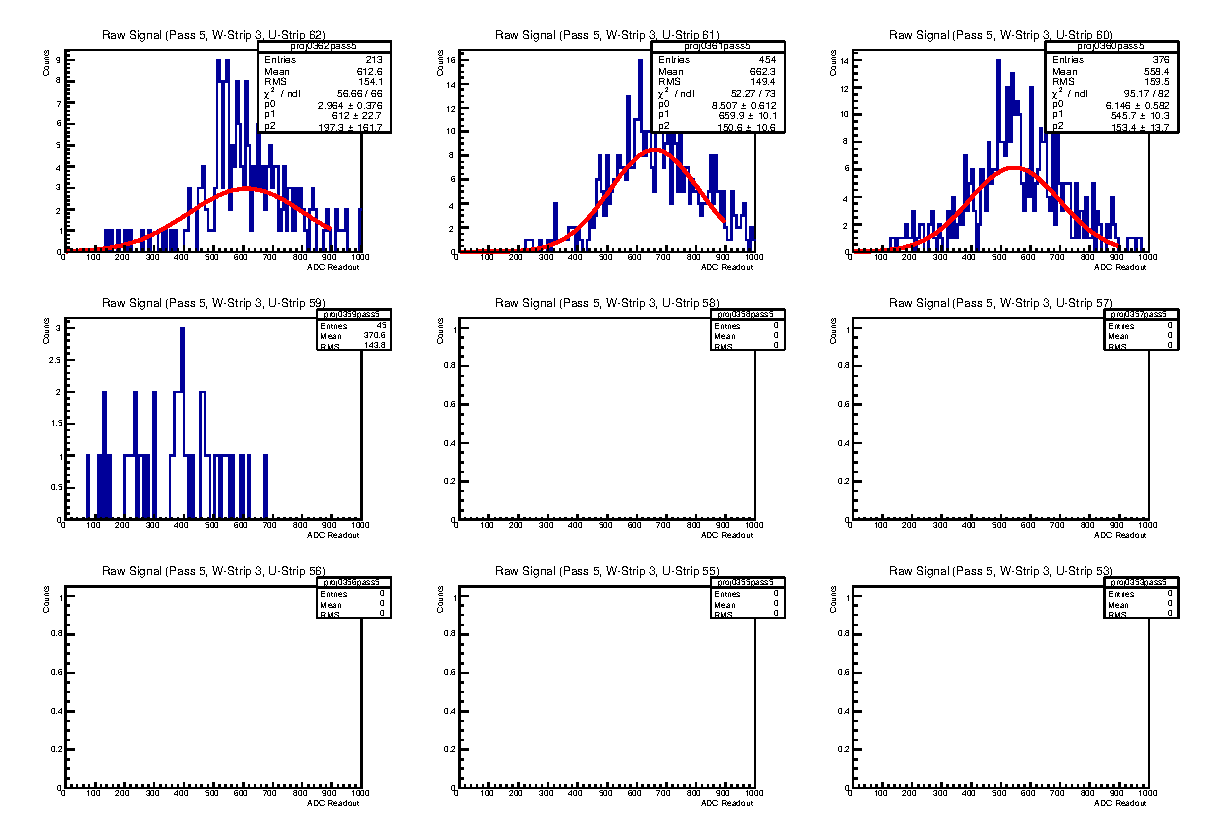
\includegraphics[width= \textwidth, keepaspectratio = true]{ustrip3}
        \caption{Shown are all of the w projections onto u-strip 3. The distribution shown peaks around 15 counts.}
        \label{fig:ustrip3}
    \end{subfigure}
    ~
    \begin{subfigure}[h]{0.4\textwidth}
        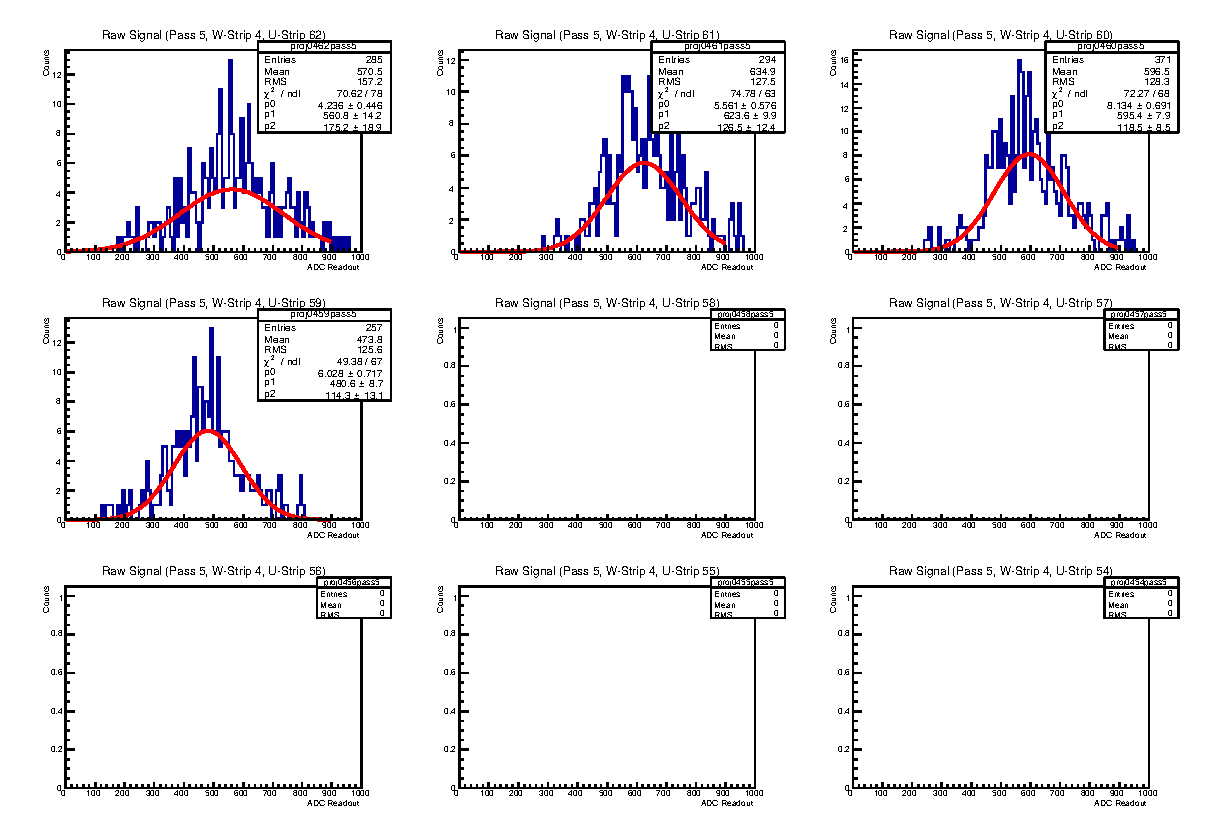
\includegraphics[width= \textwidth, keepaspectratio = true]{ustrip4}
        \caption{Shown are all of the w projections onto u-strip 4. The distribution shown peaks around 15 counts.}
        \label{fig:ustrip4}
    \end{subfigure}
    ~
    \begin{subfigure}[h]{0.4\textwidth}
        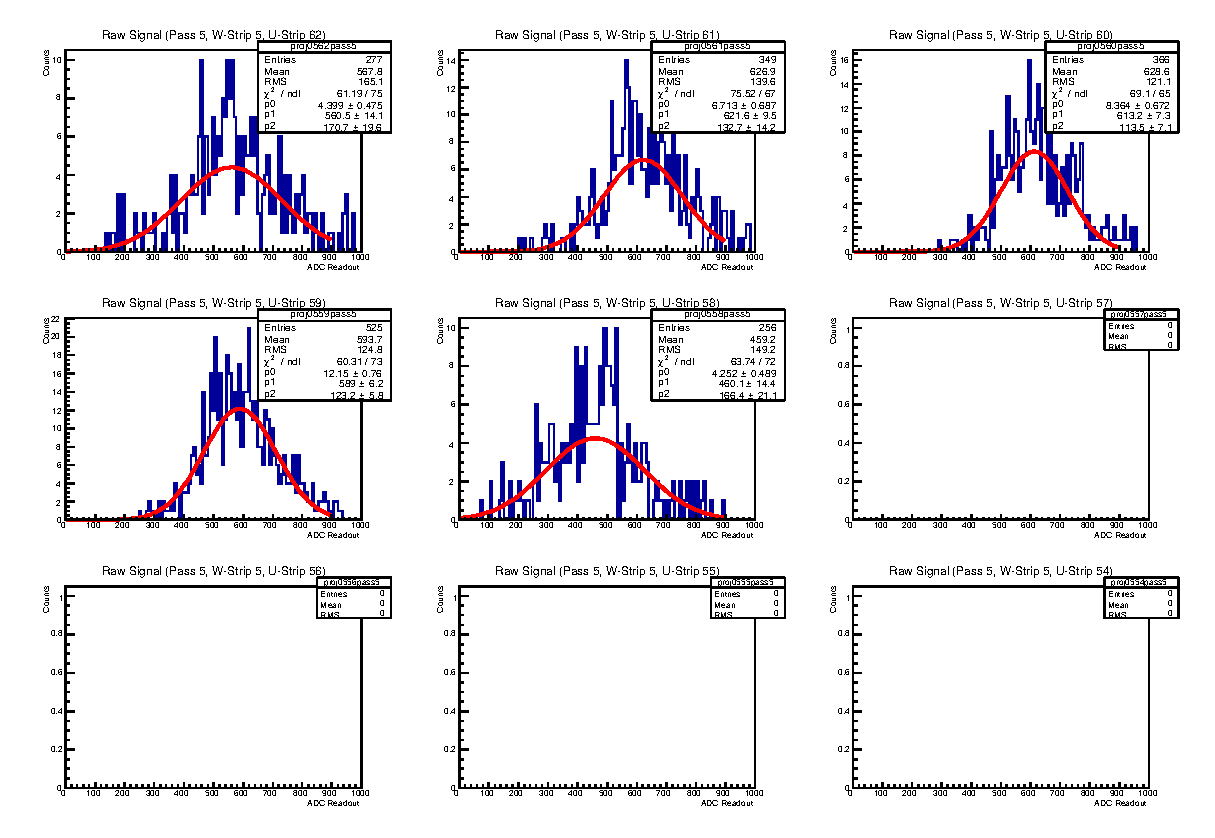
\includegraphics[width= \textwidth, keepaspectratio = true]{ustrip5}
        \caption{Shown are all of the w projections onto u-strip 5. The distribution shown peaks around 15 counts.}
        \label{fig:ustrip5}
    \end{subfigure}
    ~
    \begin{subfigure}[h]{0.4\textwidth}
        \includegraphics[width= \textwidth, keepaspectratio = true]{ustrip6}
        \caption{Shown are all of the w projections onto u-strip 6. The distribution shown peaks around 15 counts.}
        \label{fig:ustrip6}
    \end{subfigure}
    ~
    \begin{subfigure}[h]{0.4\textwidth}
        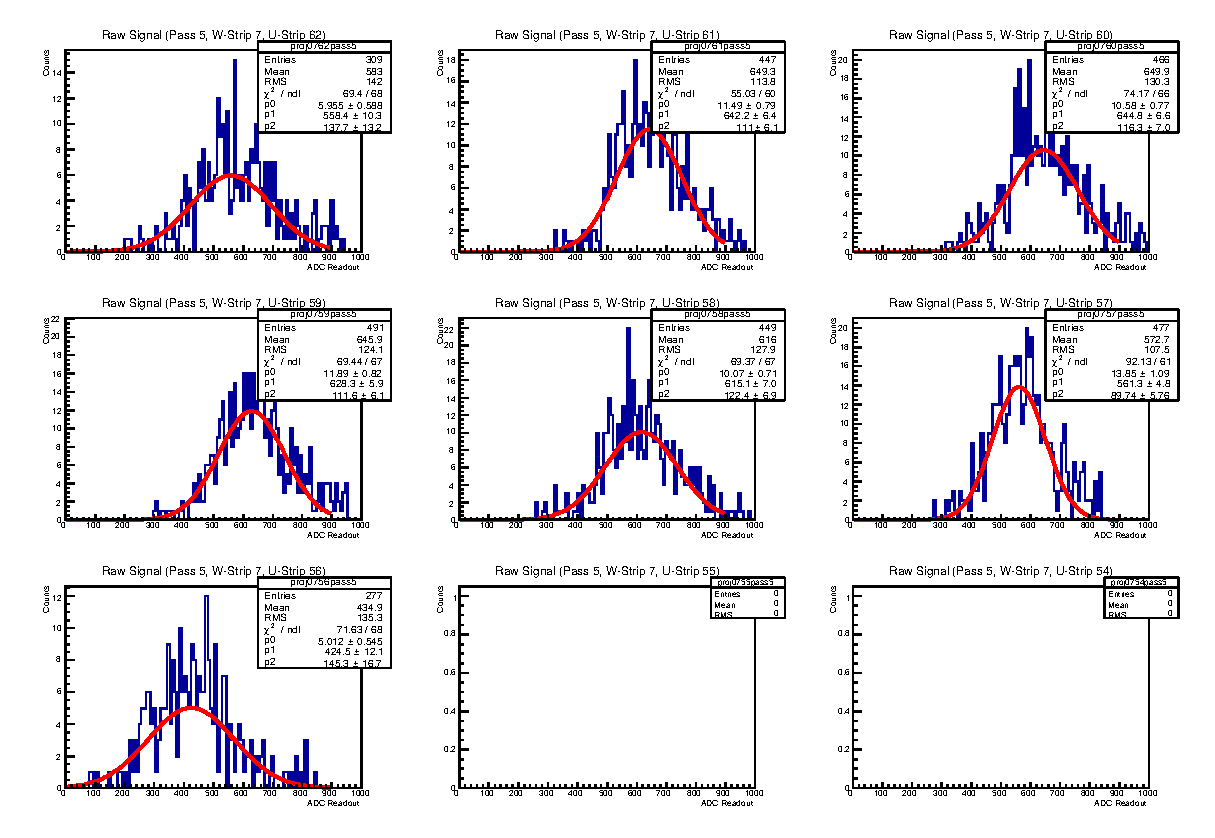
\includegraphics[width= \textwidth, keepaspectratio = true]{ustrip7}
        \caption{Shown are all of the w projections onto u-strip 7. The distribution shown peaks around 15 counts.}
        \label{fig:ustrip7}
    \end{subfigure}
    ~
    \begin{subfigure}[h]{0.4\textwidth}
        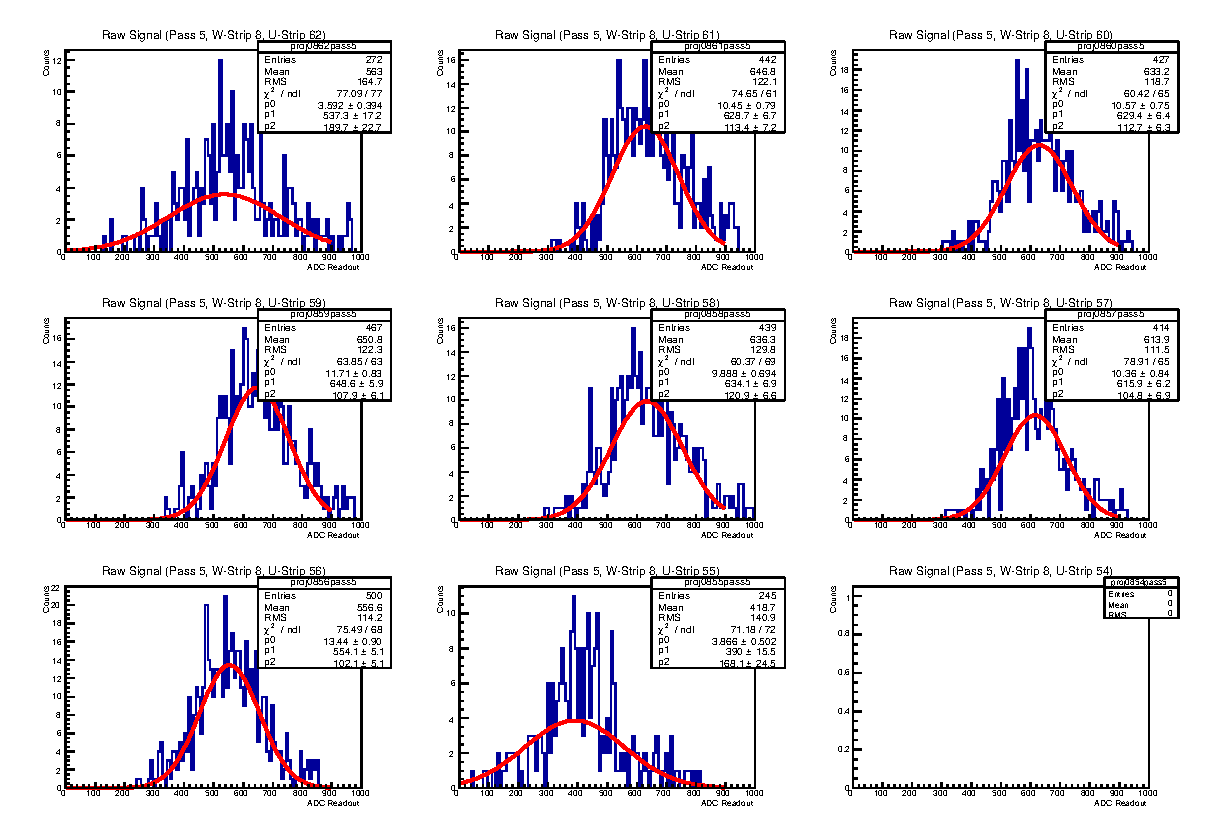
\includegraphics[width= \textwidth, keepaspectratio = true]{ustrip8}
        \caption{Shown are all of the w projections onto u-strip 8. The distribution shown peaks around 15 counts.}
        \label{fig:ustrip8}
    \end{subfigure}
    \caption{Plotted are a six of the short scintillator strips. Each subfigure shows projections of the last 9 w-strips. Therefore these plot axises are counts versus ADC value detected by the u layer PMT.}
    \label{fig:statstud1}
\end{figure}


\FloatBarrier
